% AnimatorSBT System Architecture Diagram
% Usage: Compile standalone with pdflatex, or include in main paper via:
%   \includegraphics[width=\columnwidth]{figures/architecture}
%
\documentclass[tikz,border=2mm]{standalone}

\usepackage[T1]{fontenc}
\usepackage{tikz}
\usetikzlibrary{arrows.meta, positioning, shapes.geometric, shapes.symbols, fit, calc}

\begin{document}

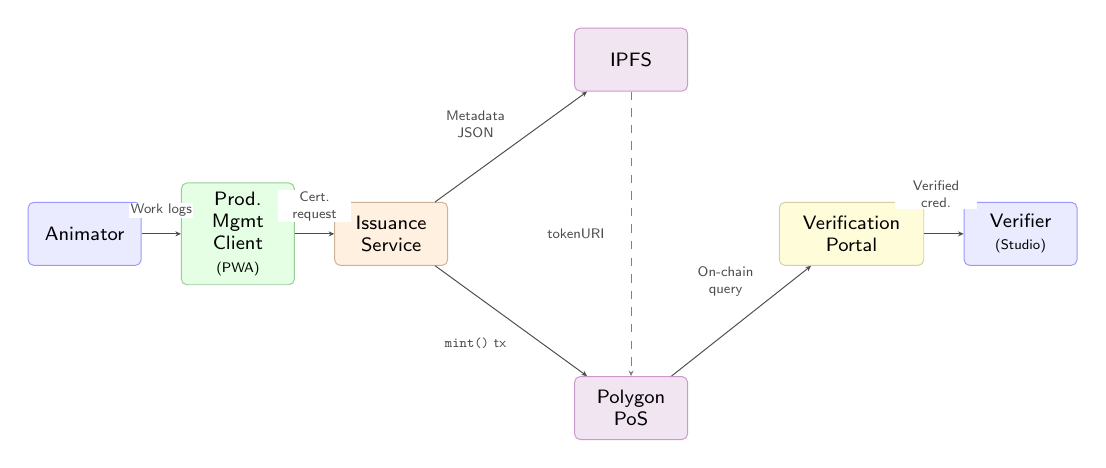
\begin{tikzpicture}[
    % --- Global styles ---
    node distance=6mm and 5mm,
    >={Stealth[length=2pt,width=1.8pt]},
    every node/.style={font=\sffamily\scriptsize},
    % --- Component boxes ---
    component/.style={
      draw, rounded corners=2pt,
      minimum height=8mm, minimum width=14mm,
      text width=12mm, align=center,
      line width=0.35pt,
    },
    % Override text width where needed
    wide component/.style={
      component, text width=16mm, minimum width=18mm,
    },
    actor/.style={component, fill=blue!8, draw=blue!40},
    pmc/.style={component, fill=green!10, draw=green!50!black!40},
    service/.style={component, fill=orange!12, draw=orange!50!black!40},
    infra/.style={component, fill=violet!10, draw=violet!40},
    portal/.style={wide component, fill=yellow!15, draw=yellow!50!black!40},
    % --- Arrow styles ---
    flow/.style={->, line width=0.35pt, draw=black!70},
    dashed flow/.style={->, line width=0.35pt, draw=black!50, dashed},
    % --- Label style ---
    lbl/.style={font=\sffamily\tiny, text=black!70, fill=white,
                inner sep=0.5pt},
  ]

  %% ---- Nodes (left to right) ----

  % Animator
  \node[actor] (animator) {Animator};

  % Production Management Client
  \node[pmc, right=of animator] (pmc)
    {Prod.\ Mgmt Client {\tiny(PWA)}};

  % Issuance Service
  \node[service, right=of pmc] (issuer)
    {Issuance Service};

  % IPFS (above, between issuer and portal)
  \node[infra, above right=14mm and 16mm of issuer] (ipfs) {IPFS};

  % Polygon PoS (below, between issuer and portal)
  \node[infra, below right=14mm and 16mm of issuer] (polygon) {Polygon PoS};

  % Verification Portal
  \node[portal, right=42mm of issuer] (portal)
    {Verification Portal};

  % Verifier
  \node[actor, right=of portal] (verifier)
    {Verifier {\tiny(Studio)}};

  %% ---- Arrows (lines only) ----

  \draw[flow] (animator) -- (pmc);
  \draw[flow] (pmc) -- (issuer);
  \draw[flow] (issuer) -- (ipfs);
  \draw[flow] (issuer) -- (polygon);
  \draw[dashed flow] (ipfs) -- (polygon);
  \draw[flow] (polygon) -- (portal);
  \draw[flow] (portal) -- (verifier);

  %% ---- Labels (placed independently to avoid overlap) ----

  \node[lbl] at ($(animator)!0.5!(pmc) + (0, 3mm)$)
    {Work logs};
  \node[lbl, text width=9mm, align=center] at ($(pmc)!0.5!(issuer) + (0, 3.5mm)$)
    {Cert.\ request};
  \node[lbl, text width=9mm, align=center] at ($(issuer)!0.45!(ipfs) + (-3mm, 4mm)$)
    {Metadata JSON};
  \node[lbl, text width=8mm, align=center] at ($(issuer)!0.45!(polygon) + (-3mm, -4mm)$)
    {\texttt{mint()} tx};
  \node[lbl] at ($(ipfs)!0.5!(polygon) + (-7mm, 0)$)
    {tokenURI};
  \node[lbl, text width=9mm, align=center] at ($(polygon)!0.5!(portal) + (-2mm, 5mm)$)
    {On-chain query};
  \node[lbl, text width=10mm, align=center] at ($(portal)!0.5!(verifier) + (0, 5mm)$)
    {Verified cred.};

\end{tikzpicture}

\end{document}
